\documentclass[a4paper,12pt]{article} % Tipo de documento y tamaño de letra.
\usepackage[utf8]{inputenc} % Para que reconozca caracteres especiales como tildes.
\usepackage[spanish]{babel} % Para definir el idioma y el formato de fechas en español.
\usepackage{amsmath, amssymb} % Paquetes para símbolos y ecuaciones avanzadas (Para hacer una ecuación con un recuadro).
\usepackage{ragged2e} % Para justificar textos.
\usepackage{multicol} % Para crear columnas.
\usepackage{slashed} % Para generar números o variables canceladas (Una línea diagonal sobre el número o variable).
\usepackage{graphicx} % Paquete para poner graficas.
\usepackage{float} % Para poder dejar la imagen en un punto fijo del documento.
\usepackage{longtable} % Para tablas largas.
\usepackage{cancel} % Para hacer cancelaciones en medio de operaciones.
\usepackage{xcolor} % Para el color y esas cosas.
\usepackage{apacite} % Paquete para citas APA.
\usepackage{fancyhdr} % Para personalizar encabezados y pies de página.
\usepackage{geometry} % Para ajustar márgenes.
\usepackage{setspace} % Para ajustar el interlineado.
\usepackage{natbib} % Para manejar las citas y que no queden pegadas y feas :P.
\usepackage{hyperref} % Para que los enlaces sean clickeables.
\usepackage[version=4]{mhchem}  % Versión recomendada para mayor funcionalidad.
\usepackage{chemfig} %También para hacer estructuras químicas.
\usepackage{array} % Para mejor control de las columnas.
\usepackage{siunitx} % Para unidades físicas.


\pagestyle{fancy}
\fancyhf{} % Limpia encabezados y pies de página predeterminados
\fancyhead[L]{\textbf{ACTIVIDAD}} % Encabezado izquierdo
\fancyhead[R]{\textbf{QUÍMICA}} % Encabezado derecho
\fancyfoot[C]{\thepage} % Número de página en el centro del pie

\geometry{headheight=12.96115pt, top=1in, bottom=1in, left=1in, right=1in}
\begin{document}


\begin{figure}[H] 
    \centering
    
\includegraphics[width=0.5\textwidth]{Unir.jpg} 
\end{figure}

\vspace{\baselineskip}

% Ajustamos manualmente todo ;)
\begin{center}
    \textbf{\Large ENLACE QUÍMICO Y GASES IDEALES } \\[0.3cm]
    \vspace{\baselineskip}
    \textbf{Liz Ángel Núñez Torres} \\[0.4cm]
    \textbf{Grado en Física} \\[0.4cm]
    \textbf{Universidad Internacional de La Rioja} \\[0.4cm]
    \textbf{19 de abril de 2025}
\end{center}


\newpage
\tableofcontents

\newpage

\section{Enlace químico.}

\begin{justify}
    \begin{itemize}
        \item En algunos compuestos que contienen elementos del tercer período o 
        sucesivos de la tabla periódica, no es aplicable regla del octeto, ¿por qué sucede esto?.
        \item Escribe la estructura de Lewis de 5 compuestos que no satisfagan la regla del octeto.
    \end{itemize}
\end{justify}

\vspace{\baselineskip}

\subsection{Solución Excepciones.}

\vspace{\baselineskip}

\begin{justify}
    Estas excepciones ocurren si se presentan las siguientes tres ocasiones (\citet{Excepciones}):
    \begin{enumerate}
        \item Moléculas con un número impar de electrones de valencia.
        \item Moléculas con pocos electrones de valencia (Octeto incompleto).
        \item Moléculas que poseen átomos con más de ocho electrones de valencia (Hipervalencia).
    \end{enumerate}
\end{justify}

\vspace{\baselineskip}

\begin{justify}
    \textbf{Número impar de electrones de valencia.}
\end{justify}
\begin{justify}
    Las moléculas o iones que contienen elementos del bloque \((d)\) frecuentemente presentan un número impar de electrones, es por esto que al intentar describirlos usando el modelo de \textbf{Lewis} no llegamos al resultado esperado para el octeto,
    como el óxido nítrico (\ce{NO}) con 5 y 6 electrones de valencia, resultando 11 en total.
    No podemos hacer encajar un número impar con el modelo de Lewis. (\cite{Octeto}).
\end{justify}

\vspace{\baselineskip}

\begin{justify}
    \textbf{Octeto incompleto.}
\end{justify}

\begin{justify}
    Esto sucede porque hay moléculas con átomos pequeños y pocos electrones de valencia, por esto no pueden alcanzar el octeto, por su deficiencia de electrones 
    en sus orbitales, como el Berilio (\ce{Be}) y el Boro (\ce{B}). (\cite{Octeto}).
\end{justify}

\vspace{\baselineskip}

\begin{justify}
    \textbf{Hipervalencia.}
\end{justify}
\begin{justify}
    Es la excepción más común a la regla del octeto, una molécula o un ion con al menos un átomo que posee más de un octeto de electrones.
    Aquellos elementos con el orbital \((d)\) vacíos en su capa de valencia les permite ``expandir'' el octeto y albergar más electrones como 
    el trióxido de azufre (\ce{SO_3}). (\cite{Octeto}).
\end{justify}

\newpage 


\subsection{Solución estructura de Lewis.}

\vspace{\baselineskip}

\begin{enumerate}
    \item \textbf{Óxido Nítrico (\ce{NO})} \(\Rightarrow\) Molécula con número impar de electrones.
    
    \chemfig{N~[::0]O}

    \item \textbf{Berilio cloruro (\ce{BeCl_2})} \(\Rightarrow\) Posee menos de un octeto (4 electrones de valencia).
    
    \chemfig{Cl-Be-Cl}

    \item \textbf{Trióxido de azufre (\ce{SO_3})} \(\Rightarrow\) Excede el octeto.
    
    \chemfig{O=[:30]S(=[:150]O)(-[:270]O)}


    \item \textbf{Hexafluoruro de azufre (\ce{SF_6})} \(\Rightarrow\) Excede el octeto con 12 electrone de valencia.
    
    \chemfig{F-[:0]S(-[:60]F)(-[:120]F)(-[:180]F)(-[:240]F)(-[:300]F)}


    \item \textbf{Trifluoruro de boro (\ce{BF_3})} \(\Rightarrow\) Tiene solamente 6 electrones de valencia.
    
    \chemfig{F-B(-F)-F}
\end{enumerate}

\vspace{\baselineskip}


\section{Gases ideales.}

\begin{justify}
    \begin{itemize}
        \item Un recipiente contiene un volumen de \(3,3 l\) de gas oxígeno a una temperatura de \(28^\circ C\); el gas ejerce una presión de \( 2,7 \; atm\). Calcula el número de moles presentes en el gas.
        \item 5,9 moles de gas monóxido de carbono están presentes en un contenedor de \(24,2 l\) de volumen, ¿cuál es la presión del gas (en psi) si la temperatura es \(42^\circ C\)? 
    \end{itemize}
\end{justify}

\vspace{\baselineskip}

\newpage

\subsection{Solución Ejercicios.}

\vspace{\baselineskip}

\begin{enumerate}
    \item Vamos organizar nuestros datos primero.
        \begin{table}[h]
        \centering
        \renewcommand{\arraystretch}{1.5} % Espaciado vertical.
        \begin{tabular}{|>{\bfseries}l|r|} % Primera columna en negrita.
        \hline
        \multicolumn{1}{|c|}{\textbf{Variable}} & \multicolumn{1}{c|}{\textbf{Valor}} \\
        \hline
        Presión \((P)\). & \SI{2.7}{atm} \\
        \hline
        Volumen \((V)\). & \SI{3.3}{\liter} \\
        \hline
        Número de moles \((n)\). & \SI{}{} \\
        \hline
        Constante universal de los gases ideales \((R)\). & \SI{0.0821}{\frac{atm \cdot \liter}{\mole \cdot \kelvin}} \\
        \hline
        Temperatura \((T)\). & \SI{301.15}{\kelvin} \\
        \hline
        \end{tabular}
        \caption{Datos sobre el gas en el recipiente.}
        \label{tab:gas_ideal}
        \end{table}

        \begin{justify}
            Para este punto vamos a usar la ecuación de la \textbf{Ley de los Gases Ideales}. 
    
            \[PV = nRT.\]
        \end{justify}
        \begin{justify}
            Dado que necesitamos saber el valor de \(n\), procedemos a despejarla.

            \[PV = nRT \Rightarrow n = \frac{PV}{RT}.\]
        \end{justify}
        \begin{justify}
            Ahora sustituimos por nuestros valores y obtenemos el resultado. (Hemos obviado la conversión de grados a Kelvin debido a la simplicidad del cálculo, que es meramente sumar 273.15 K).

            \vspace{\baselineskip}

            \[n = \frac{2.7 \cancel{atm} \cdot 3.3 \cancel{\ce{l}}}{0.0821\frac{\cancel{atm} \cdot \cancel{\ce{l}}}{mol \cdot \cancel{\ce{K}}} \cdot 301.15 \cancel{\ce{K}}} \Rightarrow n = \frac{8.91}{24.724} \cdot mol.\]

            \vspace{\baselineskip}

            \[\textcolor{blue}{\boxed{n = 0.3603 \; mol.}}\]
        \end{justify}

        \item Vamos usar el mismo procedimiento que en el putno anterior, organizaremos nuestros datos, usaremos la Ley de los gase ideales y obtendremos el resultado, resultado que pasará por una conversión de atmosferas \((atm)\) a libras por pulgada cuadrada \((PSI).\)
        \begin{table}[h]
            \centering
            \renewcommand{\arraystretch}{1.5}   
            \begin{tabular}{|>{\bfseries}l|r|} % Primera columna en negrita.
            \hline
            \multicolumn{1}{|c|}{\textbf{Variable}} & \multicolumn{1}{c|}{\textbf{Valor}} \\
            \hline
            Presión \((P)\). & \SI{}{} \\
            \hline
            Volumen \((V)\). & \SI{24.2}{\liter} \\
            \hline
            Número de moles \((n)\). & \SI{5.9}{\mole} \\
            \hline
            Constante universal de los gases ideales \((R)\). & \SI{0.0821}{\frac{atm \cdot \liter}{\mole \cdot \kelvin}} \\
            \hline
            Temperatura \((T)\). & \SI{315.15}{\kelvin} \\
            \hline
            \end{tabular}
            \caption{Datos sobre el gas en el contenedor.}
            \label{tab:gas_ideal}
            \end{table}

            \begin{justify}
                Usamos la \textbf{Ley de los Gases Ideales} y despejamos nuestra incognita.

                \[PV = nRT \Rightarrow P = \frac{nRT}{V}.\]
            \end{justify}
            \begin{justify}
                Sustituyendo por nuestros datos:

                \[P = \frac{5.9 \cancel{mol} \cdot 0.0821\frac{atm \cdot \cancel{l}}{\cancel{mole} \cdot \cancel{K}} \cdot 315.15 \cancel{K}}{24.2 \cancel{l}} \Rightarrow \frac{152.65}{24.2} \cdot \; atm \Rightarrow 6.3078 \; atm.\]
            \end{justify}

            \begin{justify}
                Ahora hacemos la conversión.

                \[1 \; atm = 14.6959 \; PSI\]

                \[\downarrow \]

                \[P = 6.3078 \cdot 14.6959\]

                \[\downarrow \]

                \[\textcolor{blue}{\boxed{P = 92.699 \; PSI.}}\]
            \end{justify}
\end{enumerate}

\newpage

\bibliographystyle{plainnat}  
\bibliography{referencias}    


\section{Calificación/Observaciones.}
\begin{figure}[H] 
    \centering
    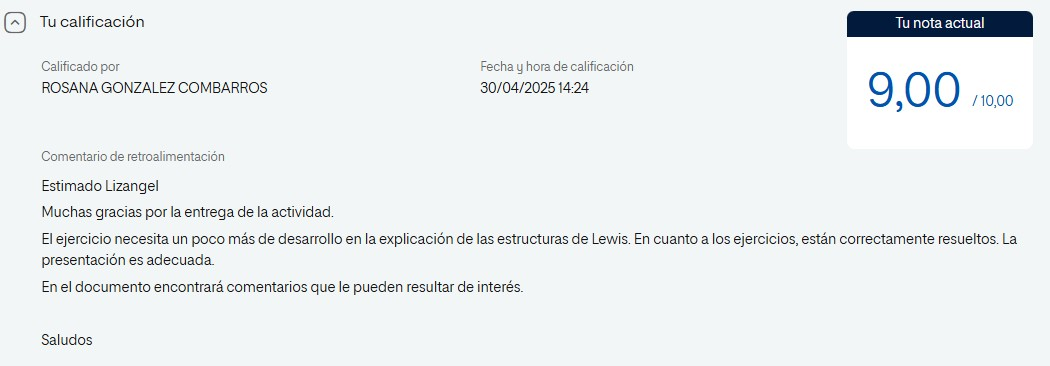
\includegraphics[width=1.1 \textwidth]{calificacion.jpg} 
\end{figure}

\end{document}